%% ---------------------------------------------------------------------------
%% Amortized learning of a survey AUV's navigation error budget
%% IEEE conference format (IEEEtran). Compile: pdflatex -> bibtex -> pdflatex x2
%%
%% Red \todo{} marks are results that do not exist yet (network training, SBC,
%% misspecification test) or facts to confirm. Every number that is not in a
%% \todo{} comes from analysis/*/results/*.md and can be regenerated with
%% analysis/scripts/run_all.sh.
%% ---------------------------------------------------------------------------
\documentclass[conference]{IEEEtran}
\IEEEoverridecommandlockouts

\usepackage{cite}
\usepackage{amsmath,amssymb,amsfonts}
\usepackage{graphicx}
\usepackage{booktabs}
\usepackage{siunitx}
\usepackage{xcolor}
\usepackage{textcomp}
\usepackage[hidelinks]{hyperref}
\usepackage{url}

\graphicspath{{figures/}}
\sisetup{detect-all, range-phrase = --, range-units = single}

\newcommand{\todo}[1]{\textcolor{red}{[TODO: #1]}}
\newcommand{\vect}[1]{\boldsymbol{#1}}
\newcommand{\btheta}{\vect{\theta}}
\newcommand{\bx}{\vect{x}}
\newcommand{\Rz}{\mathbf{R}_z}

\begin{document}

\title{Amortized Learning of a Survey AUV's Navigation Error Budget from One Surface Star Pattern}

\author{\IEEEauthorblockN{Abubakar Aliyu Badawi}
\IEEEauthorblockA{\textit{Department of Marine Technology} \\
\textit{Norwegian University of Science and Technology (NTNU)}\\
Trondheim, Norway \\
\todo{institutional e-mail}}
}

\maketitle

\begin{abstract}
Every sounding, sidescan pixel and water-column sample collected by an autonomous underwater vehicle (AUV) inherits the error of the vehicle's dead-reckoned position. That error is governed by a few slowly varying parameters, chiefly heading bias, speed-scale error and the ambient current, which are usually calibrated once and reported as point estimates. This paper learns an amortized posterior over them with simulation-based inference: a summary network and a normalizing flow are trained on a purely kinematic simulator and applied, without retraining, to \SI{120}{\second} windows of real sensor data. The data come from a field campaign in Svalbard in September 2026, where a Light AUV (LAUV) flew a surface star pattern on six headings and, the next day, a \SI{34}{\minute} sidescan dive; a second vehicle without bottom lock serves as an out-of-configuration case. On held-out simulations the posterior is well calibrated (90\,\% intervals contain the truth in 92--94\,\% of cases). On 23 real star windows the posterior mean of the heading bias follows an independent per-window estimate from bottom track and GPS (correlation 0.93; estimate inside the 90\,\% interval in 21 of 23 windows) and reveals a heading-dependent compass bias between $-2.6^{\circ}$ and $+3.4^{\circ}$ that a single constant cannot represent. Against constant least-squares references the intervals are too narrow (52--78\,\% containment), and a first noise model was overconfident until GPS and bottom-track noise were made broad nuisance parameters. Propagated through the sidescan dive, the posterior over-predicts the closure error (\SIrange{56}{83}{\meter} predicted, \SI{23}{\meter} observed with about \SI{16}{\meter} endpoint uncertainty). For the second vehicle, whose two dives closed \SI{224}{\meter} and \SI{298}{\meter} off in water-track dead reckoning, the predicted 90\,\% intervals are wide and contain both closures, whereas a Mahalanobis test in summary space flags none of the dive windows. Amortized calibration from surface windows is feasible; using it to predict underwater error is not yet supported, and summary-space distance is not a sufficient misspecification test here.
\end{abstract}

\begin{IEEEkeywords}
autonomous underwater vehicle, dead reckoning, navigation error, simulation-based inference, amortized Bayesian inference, model misspecification, sidescan georeferencing
\end{IEEEkeywords}

%% ===========================================================================
\section{Introduction}
%% ===========================================================================

An AUV below the surface has no access to GNSS and navigates by dead reckoning: a heading from a magnetic attitude and heading reference system (AHRS) or an inertial unit, a speed through water or over ground from a Doppler velocity log (DVL) or a propeller model, and a depth from pressure \cite{paull2014review}. The position estimate drifts with time, and every payload measurement is georeferenced with that drifting estimate. AUV sidescan and multibeam surveys, including archaeological work in the Arctic \cite{ludvigsen2016integrated,mogstad2020figaro}, depend on this georeferencing: a target seen in a mosaic is located only as well as the vehicle was, and mosaics from reciprocal survey lines fail to overlay when heading or scale errors are present.

The error budget of such a system is dominated by a few slowly varying quantities: a constant heading offset between the sensed and true heading, a multiplicative error on the speed source, and the horizontal current, which adds to the velocity through water but not to the velocity over ground. Kinsey and Whitcomb \cite{kinsey2007alignment} estimate the Doppler--attitude alignment in situ by least squares against reference navigation data; Hegren{\ae}s and Hallingstad \cite{hegrenaes2011modelaided} estimate the current online inside a model-aided inertial navigation system. Both return point estimates with a covariance that is only as good as the linearisation and the Gaussian noise assumption behind it.

This paper asks a different question: can a network trained on simulations alone return a \emph{calibrated} posterior over these parameters from a short window of raw sensor data, so that a supervisor can quote a position-uncertainty envelope along a survey rather than a single closure number? The tool is amortized simulation-based inference (SBI) \cite{cranmer2020frontier,greenberg2019apt}: a simulator generates parameter--observation pairs, a summary network compresses the observation and a normalizing flow learns the posterior \cite{radev2022bayesflow,radev2023joss}. Once trained, inference on a new window costs a forward pass. Calibration is tested with simulation-based calibration (SBC) \cite{talts2018sbc}, and the network's own summary statistics provide a test for whether an observation lies outside what it was trained on \cite{schmitt2023misspecification}.

Three questions are put to field data from Svalbard, and the answers are reported whichever way they fall.
\begin{enumerate}
  \item Are the parameters identifiable from a two-minute window, and is the amortized posterior calibrated, on simulations and on real surface windows with independent references?
  \item Does a posterior calibrated at the surface predict the dead-reckoning error of a real submerged survey, so that a position-uncertainty envelope can be attached to the payload data?
  \item When the vehicle or its sensors differ from what the simulator assumed, does the posterior widen, or does a misspecification test flag the windows?
\end{enumerate}

The contribution is not a new inference algorithm. It is a worked field example, failures included: a first noise model that passed calibration on simulations but was overconfident on real data and was diagnosed and replaced; a heading-dependent compass bias that the single-constant model of the classical calibration cannot express, and that the posterior recovers; the observation that a current fitted at one site cannot be carried to another and must not be propagated as if it could; and a misspecification test in summary space that does not separate the vehicle and configuration it was meant to.

%% ===========================================================================
\section{Field Data}
%% ===========================================================================

\subsection{Campaign and vehicles}

The data were collected during the AT-334/834 field course of the University Centre in Svalbard on 7--8 September 2026 in Isfjorden, Svalbard. Two LAUV-class vehicles \cite{sousa2012lauv} were operated: \emph{LAUV Marie} (sidescan, multibeam, CTD, Nortek DVL500, Microstrain AHRS, GPS) and \emph{LAUV Thor} (CTD, fluorometer, turbidity, Nortek DVL, Microstrain AHRS, GPS). Both run the DUNE onboard software of the LSTS toolchain \cite{pinto2013lsts} and log every internal message in the IMC format \cite{martins2009imc}. Marie ran DUNE 2025.06 with IMC 5.5; Thor ran DUNE 2020.11 with IMC 5.4. The difference matters below.

Three logs are used (Table~\ref{tab:logs}). The star mission and Thor's water-column mission were flown simultaneously on 7 September in Adolfbukta, inner Billefjorden, about \SI{2}{\kilo\meter} in front of Nordenskiöldbreen; the sidescan survey was flown on 8 September over a helicopter wreck in Adventfjorden, about \SI{50}{\kilo\meter} away. No ultra-short-baseline (USBL) fix reached any vehicle: the logs contain only acoustic text requests from the ship-side gateway, and the vehicles were configured with the USBL node disabled. All position truth in this paper therefore comes from the vehicles' own standalone GPS receivers at the surface.

\begin{table}[t]
\caption{Logs used. Duration is the log length; GPS is the share of 1\,Hz fixes accepted by the navigation filter (valid position, horizontal accuracy $<\SI{15}{\meter}$, HDOP $<4$).}
\label{tab:logs}
\centering
\small
\setlength{\tabcolsep}{4pt}
\begin{tabular}{@{}lllrrr@{}}
\toprule
Log & Vehicle & Site & Dur.\ [min] & GPS [\%] & Dives \\
\midrule
Star & Marie & Adolfbukta & 13.2 & 100 & 0 \\
Yoyo & Thor & Adolfbukta & 53.8 & 15 & 2 \\
Sidescan & Marie & Adventfj. & 34.9 & 1.9 & 1 \\
\bottomrule
\end{tabular}
\end{table}

\subsection{Sensor streams}

The streams used, at their native rates, are GPS fix (\SI{1}{\hertz}; position, course and speed over ground, accuracy estimate, HDOP, validity bits), AHRS Euler angles (\SI{50}{\hertz}), DVL bottom-track and water-track velocity in the vehicle frame (\SI{5}{\hertz}, per-sample validity), propeller speed (\SI{10}{\hertz}), CTD depth, the filter's state estimate (\SI{20}{\hertz}) and the vehicle-medium flag. Timestamps are the vehicle clock, which is GPS-synchronised; the GPS message additionally carries the UTC time of fix, which lags the vehicle timestamp by \SI{0.32}{\second} on Marie (GPS over TCP) and leads it by \SI{0.02}{\second} on Thor. The UTC time of fix is used as the epoch of each fix.

Three properties of the logs shape the analysis. First, the AHRS yaw in the log equals its own magnetic-yaw field, so it is a magnetic heading; the filter's state estimate carries a constant offset of \SI{12.72}{\degree} (Marie, 7 September), \SI{12.74}{\degree} (Marie, 8 September) and \SI{14.03}{\degree} (Thor) relative to it. The size is that of the local magnetic declination: the World Magnetic Model 2025 \cite{chulliat2025wmm} gives \SI{14.02}{\degree} at the star site and \SI{14.00}{\degree} at Thor's position on 7 September, and \SI{12.86}{\degree} at the sidescan site on 8 September. Thor's offset matches the model; Marie's is \SI{1.3}{\degree} smaller at the star site, and the reason was not established. Second, the GPS receiver keeps emitting positions flagged valid at \SI{60}{\meter} depth, with accuracy estimates of hundreds of metres and three satellites; the filter rejects them, and so does this analysis. Third, Thor's DVL had no bottom lock in the \SIrange{70}{80}{\meter} deep fjord and its water track was flagged invalid \SI{99.7}{\percent} of the time; the flagged values are nonetheless physical (correlation 0.92 with propeller speed) and are used here as a speed source, whereas the onboard filter fell back to a propeller-speed model.

\subsection{Star mission}

The star (Fig.~\ref{fig:star_track}) consists of eight straight legs of \SIrange{104}{212}{\meter} on six distinct headings (\SIlist{305;333;96;208;338;92;209;135}{\degree} after declination), flown at \SI{1.5}{\meter\per\second} over ground with the vehicle at the surface throughout (medium flag \emph{water} for all 790 samples; CTD depth \SI{-0.29}{\meter}). The GPS delivered a fix every second with a median horizontal accuracy estimate of \SI{1.2}{\meter} and 17 satellites. The seabed lay at \SIrange{33}{73}{\meter}, within DVL range, so bottom track (\SI{98.3}{\percent} valid), water track (\SI{98.1}{\percent}) and propeller speed are all available simultaneously with GPS. This is the calibration set.

\begin{figure}[t]
\centering
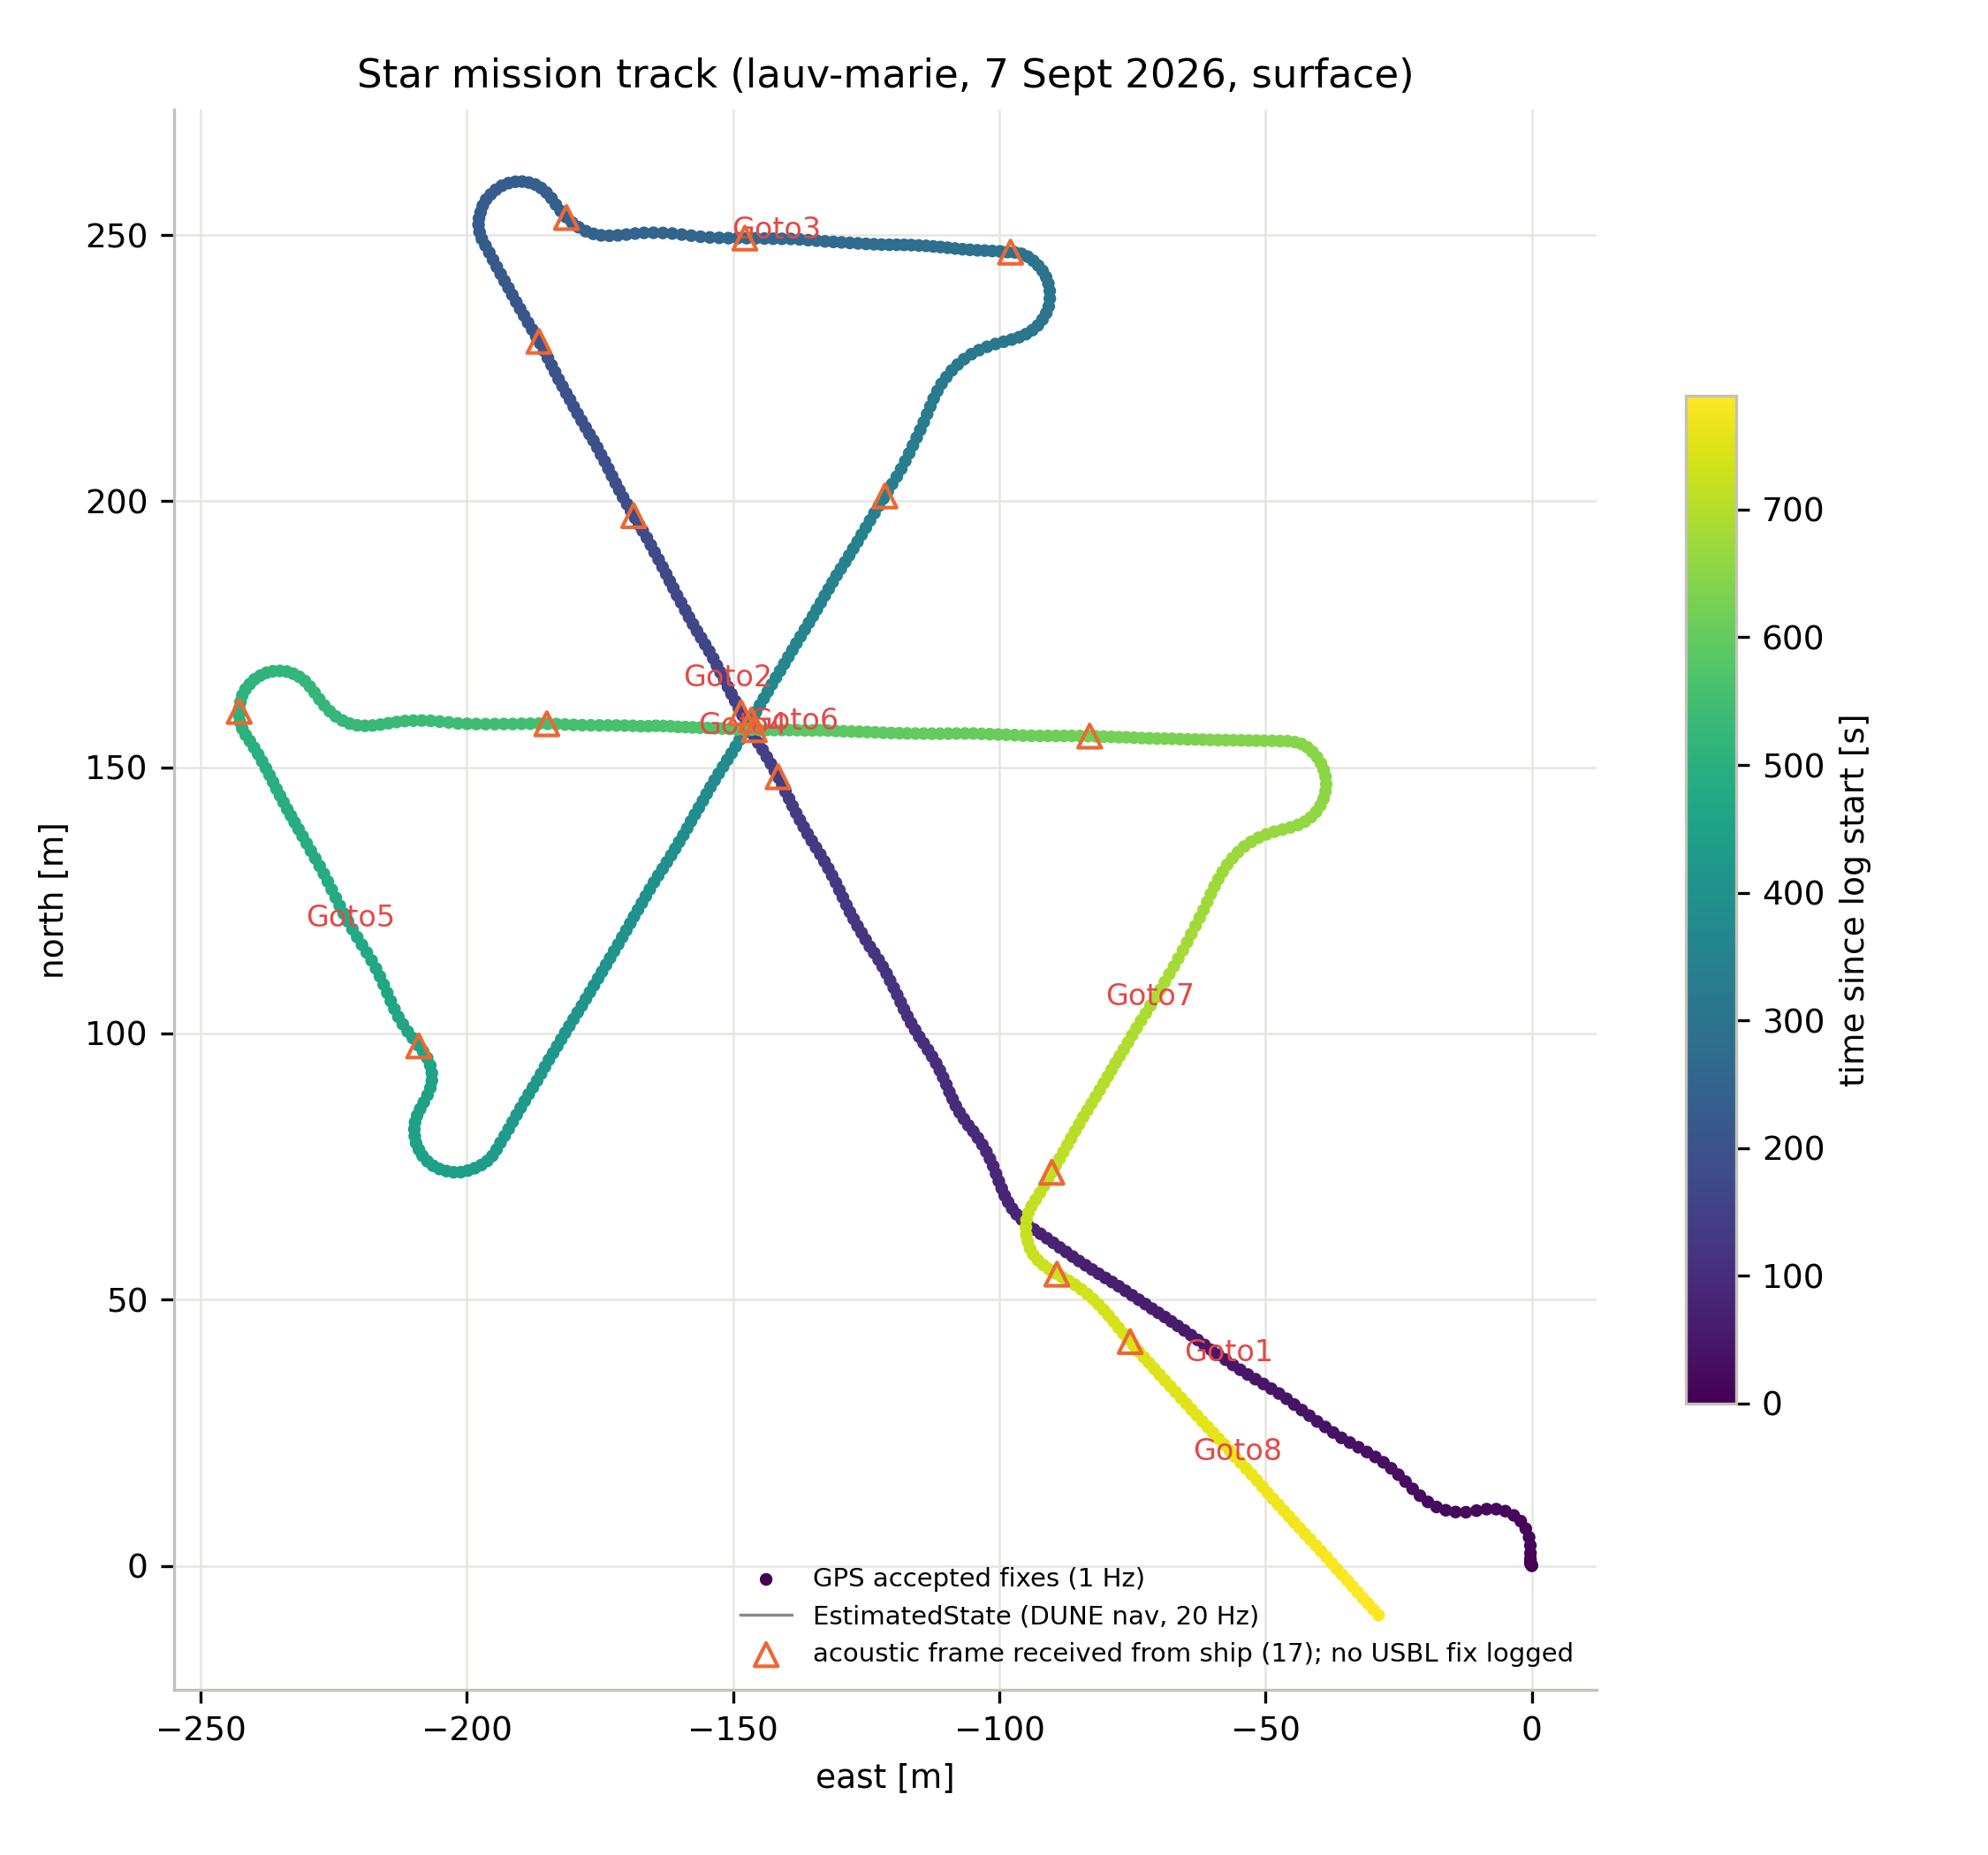
\includegraphics[width=\columnwidth]{star_track}
\caption{Star mission track of LAUV Marie at the surface, 7 September 2026, coloured by time. Triangles mark the 17 acoustic frames received from the ship; none carried a position fix.}
\label{fig:star_track}
\end{figure}

\subsection{Diving missions}

The sidescan survey dived at 07:50:25 UTC, ran an elevator to \SI{25}{\meter} and then \SI{60}{\meter}, flew nine lawnmower lines at \SI{7}{\meter} altitude and popped up at 08:24:37 after \SI{34.2}{\minute} submerged and \SI{2.73}{\kilo\meter} of path. Bottom lock was held for \SI{98.6}{\percent} of the dive (longest dropout \SI{20}{\second}). Thor's mission contained two yoyo dives of \SI{19.0}{\minute} and \SI{24.7}{\minute} (GPS gaps of \SI{20.8}{\minute} and \SI{24.9}{\minute}) between surface runs of \SIrange{2}{4}{\minute} on headings between \SI{290}{\degree} and \SI{330}{\degree}.

%% ===========================================================================
\section{Method}
%% ===========================================================================

\subsection{Parameters}

The latent vector is
\begin{equation}
\btheta = (\delta,\; s,\; c_N,\; c_E,\; \sigma_v),
\end{equation}
where $\delta$ is the heading bias (true heading minus sensed heading, positive clockwise), $s$ the multiplicative error on the speed source (water track or, when the DVL is unavailable, the propeller-to-speed factor), $(c_N, c_E)$ the horizontal current in the earth frame, and $\sigma_v$ the standard deviation of the velocity measurement noise. The current is kept in Cartesian rather than polar form so that a weak current does not produce an unidentifiable direction. Optionally a DVL dropout probability is added when the validity mask is part of the observation.

Each parameter enters the over-ground velocity differently, and that is what makes them separable. With $\vect{v}_w$ the measured velocity through water in the vehicle frame, $\psi$ the sensed heading and $\Rz(\cdot)$ the rotation about the vertical,
\begin{equation}
\vect{v}_{\mathrm{og}} = s\,\Rz(\psi + \delta)\,\vect{v}_w + \vect{c}.
\label{eq:model}
\end{equation}
A heading bias rotates the body velocity and therefore produces an over-ground error that turns with the vehicle; a current adds a fixed earth-frame vector; a scale error stretches along the heading. On a single straight leg the three are confounded: a bias and a current can produce the same over-ground velocity. On legs spanning several headings they are not. This is why the star pattern, and not a straight transit, is the calibration manoeuvre, and why Thor's surface runs on nearly parallel headings are an intrinsically poor calibration set.

\subsection{Observation window}

An observation $\bx$ is a window of $T=\SI{120}{\second}$ at \SI{1}{\hertz} with twelve channels,
\begin{equation}
\begin{aligned}
\bx_t = \big(&\cos\psi_t,\ \sin\psi_t,\ u_t,\ v_t,\ n_t,\ v^{\mathrm{gps}}_{N,t},\ v^{\mathrm{gps}}_{E,t},\\
&m^{\mathrm{dvl}}_t,\ m^{\mathrm{gps}}_t,\ u^{\mathrm{bt}}_t,\ v^{\mathrm{bt}}_t,\ m^{\mathrm{bt}}_t\big),
\end{aligned}
\end{equation}
where $(u,v)$ is the DVL water-track velocity in the vehicle frame, $n$ the propeller speed in thousands of rpm, $(v^{\mathrm{gps}}_N, v^{\mathrm{gps}}_E)$ the GPS velocity over ground, $(u^{\mathrm{bt}}, v^{\mathrm{bt}})$ the DVL bottom-track velocity and $m^{(\cdot)}$ validity masks. An absent channel is zero with mask zero, in the simulation and in the real windows alike. Underwater the GPS channels are absent, so the same network handles surface and submerged windows and the posterior widens accordingly; where bottom track is present, bottom minus water track measures the current in the vehicle frame and keeps $\vect{c}$ identifiable without GPS. Real windows are cut from the logs with a stride of \SI{30}{\second}: 23 on the star, 64 on the sidescan dive, 6 on Thor's surface runs and 79 on Thor's dives, plus the 23 star windows rebuilt with the raw magnetic heading. Channels are standardised with the training statistics.

\subsection{Kinematic simulator}

The simulator is deliberately free of hydrodynamics. A heading programme $\psi^{\mathrm{true}}_t$ and a propeller programme $n_t$ are either replayed from a \SI{120}{\second} cut of the field logs, rotated by a random angle so that the network cannot memorise absolute headings, or drawn synthetically as a piecewise-constant heading with turns at \SI{10}{\degree\per\second} and a constant propeller speed; the two sources are mixed one to one. The true speed through water is $u^{\mathrm{true}}_t = k\,n_t$ with a per-window factor $k \sim \mathcal{U}(0.95, 1.35)\times10^{-3}\,\si{\meter\per\second}$ per rpm, plus a first-order autoregressive sway of \SI{0.03}{\meter\per\second}. The over-ground velocity is $\Rz(\psi^{\mathrm{true}}_t)[u^{\mathrm{true}}_t, v^{\mathrm{true}}_t]^\top + \vect{c}$. Measurements are formed as
\begin{align}
\psi_t &= \psi^{\mathrm{true}}_t - \delta + \epsilon^\psi_t, \\
(u_t, v_t) &= (u^{\mathrm{true}}_t,\ v^{\mathrm{true}}_t)/s + \vect{\epsilon}^{v}_t, \\
\vect{v}^{\mathrm{gps}}_t &= \vect{v}_{\mathrm{og},t} + \vect{\epsilon}^{\mathrm{gps}}_t,
\end{align}
with $\epsilon^\psi_t \sim \mathcal{N}(0, (\SI{0.3}{\degree})^2)$, $\vect{\epsilon}^{v}_t \sim \mathcal{N}(0, \sigma_v^2 \mathbf{I})$ and $\vect{\epsilon}^{\mathrm{gps}}_t \sim \mathcal{N}(0, \sigma_{\mathrm{gps}}^2\mathbf{I})$. Bottom track is the over-ground velocity rotated into the true vehicle frame with noise $\sigma_{\mathrm{bt}}$. DVL dropouts occur in bursts with a per-window probability drawn from $\mathcal{U}(0, 0.08)$ per second; GPS is present in \SI{60}{\percent} of the windows and bottom track in \SI{70}{\percent}. The rpm factor $k$, the dropout rate, the availability flags and the two noise levels $\sigma_{\mathrm{gps}} \sim \log\mathcal{U}(0.03, 0.25)$ and $\sigma_{\mathrm{bt}} \sim \log\mathcal{U}(0.01, 0.15)\,\si{\meter\per\second}$ are nuisances that are sampled per window but not inferred. Dead-reckoned position is a deterministic function of $(\bx, \btheta)$, so the position uncertainty along a dive is obtained by pushing posterior samples through the recorded window sequence; nothing about position is learned by the network.

This is the second version of the noise model. The first fixed $\sigma_{\mathrm{gps}} = \SI{0.05}{\meter\per\second}$, tied $\sigma_{\mathrm{bt}} = \sigma_v/2$ and started the prior of $\sigma_v$ at \SI{0.05}{\meter\per\second}. It passed calibration on simulations and was overconfident on the real star; Section~\ref{sec:v1v2} gives the diagnosis. Both versions are reported, and the ranges of the second were chosen broad, not fitted to the star.

Priors are uniform and wide enough to contain everything observed in the campaign:
\begin{equation}
\begin{aligned}
\delta &\sim \mathcal{U}(-15, 15)^{\circ}, \qquad s \sim \mathcal{U}(0.8, 1.1),\\
c_N, c_E &\sim \mathcal{U}(-0.4, 0.4)\,\si{\meter\per\second},\\
\log_{10}\sigma_v &\sim \mathcal{U}(\log_{10} 0.01, \log_{10} 0.5).
\end{aligned}
\end{equation}

\subsection{Networks, calibration test and misspecification test}

A time-series transformer summary network (two attention blocks of width 64, four heads) maps $\bx$ to a 32-dimensional summary $\vect{h}$, and an affine coupling flow with six blocks learns $q(\btheta \mid \vect{h})$, following the BayesFlow workflow \cite{radev2022bayesflow,radev2023joss}. Training is offline on \num{40000} simulations with \num{4000} held out, for 40 epochs with batches of 128 and AdamW under a cosine schedule (the BayesFlow defaults); it takes about 1.5 hours on a 20-core CPU.

Calibration is tested with SBC \cite{talts2018sbc} on \num{1000} held-out simulations with 500 posterior draws each: the rank of the true $\btheta$ among the draws must be uniform, which is checked with rank histograms, the maximum deviation of the rank ECDF from uniform, and the empirical coverage of the 50\,\% and 90\,\% central intervals. Misspecification is tested as in \cite{schmitt2023misspecification}: the squared Mahalanobis distance of $\vect{h}$ from the distribution of summaries of \num{4000} training simulations, with the threshold at the 99th percentile of the distances of \num{2000} held-out simulations. A window beyond that threshold is one on which the posterior should not be trusted, whatever its width.

\subsection{Reference values and validation protocol}

Reference values for $\btheta$ on the star are obtained by Gauss--Newton on \eqref{eq:model} over all GPS epochs, with the GPS velocity from the receiver's course and speed over ground and the DVL velocity rotated to the earth frame with the full roll--pitch--yaw rotation, averaged in \SI{\pm 0.5}{\second} bins around each fix. Only DVL samples with all three components flagged valid are used, and nothing is smoothed. The same fit with the rotation omitted gives a residual of \SI{2.14}{\meter\per\second} against \SI{0.17}{\meter\per\second} with it, which confirms the vehicle-frame convention of the DVL messages.

Four tiers of validation are used: (i) SBC on the simulator; (ii) the posterior on the real star windows against the all-leg reference, against an independent per-window heading bias obtained afterwards from bottom track and GPS (a post hoc check, marked as such), and posterior-predicted versus observed drift of the nominal dead reckoning over each window; (iii) propagation of posteriors through the recorded sidescan dive and through Thor's two dives, compared with the observed closures at resurfacing; (iv) the Mahalanobis test on Thor windows and on Marie windows fed with the raw magnetic heading. Windows are cut from the logs every \SI{30}{\second}, so neighbouring windows overlap by \SI{75}{\percent} and the 23 star windows are not independent.

Dead reckoning, whenever it is computed in this paper, is forward Euler at the DVL sample times with the vehicle-frame velocity rotated by the filter's heading; an invalid DVL sample holds the last valid one, which is what the onboard filter does within its timeout.

%% ===========================================================================
\section{Results}
%% ===========================================================================

\subsection{Identifiability on the star}

Table~\ref{tab:fits} gives the joint fits. With the filter's heading (AHRS plus the offset), the residual heading bias is $\SI{0.09}{\degree} \pm \SI{0.16}{\degree}$ from the water track and $\SI{0.03}{\degree} \pm \SI{0.16}{\degree}$ from the bottom track; the current is $(+0.003, -0.019)\,\si{\meter\per\second} \pm 0.004$; the water-track scale is $0.965 \pm 0.003$ and the bottom-track scale $0.992 \pm 0.003$; the propeller factor is 0.841 times the configured \num{1.3e-3} \si{\meter\per\second} per rpm. Adding $\delta$ and $s$ to the current-only fit lowers the residual only from 0.179 to \SI{0.171}{\meter\per\second}, which is the honest statement that on this vehicle, on this day, the heading was already right and the current was absent. Per-leg current estimates scatter around zero with magnitudes of \SIrange{0.04}{0.13}{\meter\per\second} and no preferred direction; the DVL-only estimate, bottom track minus water track, agrees at \SIrange{0.03}{0.05}{\meter\per\second}.

\begin{table}[t]
\caption{Joint least-squares fits of \eqref{eq:model} on the star, 784 GPS epochs. Uncertainties are $1\sigma$ from the residuals.}
\label{tab:fits}
\centering
\small
\begin{tabular}{@{}llrrrrr@{}}
\toprule
Input & Params & $c_N$ & $c_E$ & $\delta$ [\si{\degree}] & $s$ & RMS \\
\midrule
water tr. & $\vect{c}$ & $+0.004$ & $-0.018$ & -- & -- & 0.179 \\
water tr. & $\vect{c},\delta,s$ & $+0.003$ & $-0.019$ & $+0.09$ & 0.965 & 0.171 \\
bottom tr. & $\vect{c},\delta,s$ & $+0.006$ & $-0.006$ & $+0.03$ & 0.992 & 0.166 \\
rpm & $\vect{c},\delta,s$ & $-0.011$ & $-0.058$ & $-0.08$ & 0.841 & 0.209 \\
\midrule
\multicolumn{7}{@{}l}{\emph{raw magnetic heading (offset omitted)}} \\
water tr. & $\vect{c}$ & $+0.008$ & $-0.022$ & -- & -- & 0.386 \\
water tr. & $\vect{c},\delta,s$ & $+0.003$ & $-0.019$ & $+12.81$ & 0.965 & 0.172 \\
\bottomrule
\end{tabular}
\end{table}



The lower half of Table~\ref{tab:fits} is the cautionary case. With the raw magnetic heading, a current-only model still converges, its residual doubles, and on every leg it returns a ``current'' of \SIrange{0.33}{0.48}{\meter\per\second} whose direction is \SIrange{10}{20}{\degree} off the vehicle's beam. A single leg cannot distinguish this from a real current; the star can, and the $(\vect{c}, \delta, s)$ fit recovers $\delta = \SI{12.81}{\degree} \pm \SI{0.17}{\degree}$, within \SI{0.1}{\degree} of the \SI{12.72}{\degree} offset the onboard filter applies. This is the failure a current-only calibration would miss; a model with $\delta$ in the parameter vector recovers it (Section~IV-F).

\subsection{Drift under replayed GPS outages}

Dead reckoning was restarted from the GPS position every \SI{10}{\second} of the star and compared with GPS after \SIlist{2;5;10}{\minute} (Fig.~\ref{fig:drift}, Table~\ref{tab:drift}). With the filter's heading and the DVL water track, the median drift is \SI{4.7}{\meter} at \SI{2}{\minute} and \SI{8.5}{\meter} at \SI{10}{\minute}, about \SI{0.9}{\percent} of distance. Applying the fitted $(\delta, s, \vect{c})$ brings this to \SIrange{2.3}{3.4}{\meter}, essentially the bottom-track level, so the remaining drift is the water-track scale error, not the current. The propeller model with the configured factor drifts \SIrange{23}{40}{\meter}; with the fitted factor \SIrange{6}{29}{\meter}. The raw magnetic heading drifts \SIrange{26}{28}{\meter} at all horizons, with a large spread that depends on where in the pattern the outage starts. Only 19 ten-minute windows fit in the mission, so that column is indicative.

\begin{table}[t]
\caption{Replayed GPS outages on the star: median and maximum $|\mathrm{DR} - \mathrm{GPS}|$ in metres over all start times (every \SI{10}{\second}; windows overlap).}
\label{tab:drift}
\centering
\small
\setlength{\tabcolsep}{4pt}
\begin{tabular}{@{}lccc@{}}
\toprule
DR input & 2 min & 5 min & 10 min \\
\midrule
water track & 4.7 / 12.0 & 5.8 / 14.7 & 8.5 / 19.0 \\
bottom track & 2.2 / 8.1 & 3.2 / 6.0 & 4.3 / 7.0 \\
rpm, configured factor & 23.4 / 34.4 & 25.7 / 58.5 & 40.2 / 69.8 \\
rpm, fitted factor & 5.8 / 16.7 & 14.7 / 18.7 & 28.5 / 32.2 \\
water tr.\ $+$ fitted $(\delta,s,\vect{c})$ & 2.3 / 7.2 & 2.0 / 7.2 & 3.4 / 7.6 \\
water tr., raw magn.\ heading & 28.1 / 49.7 & 25.6 / 59.4 & 26.6 / 68.8 \\
\bottomrule
\end{tabular}
\end{table}

\begin{figure*}[t]
\centering
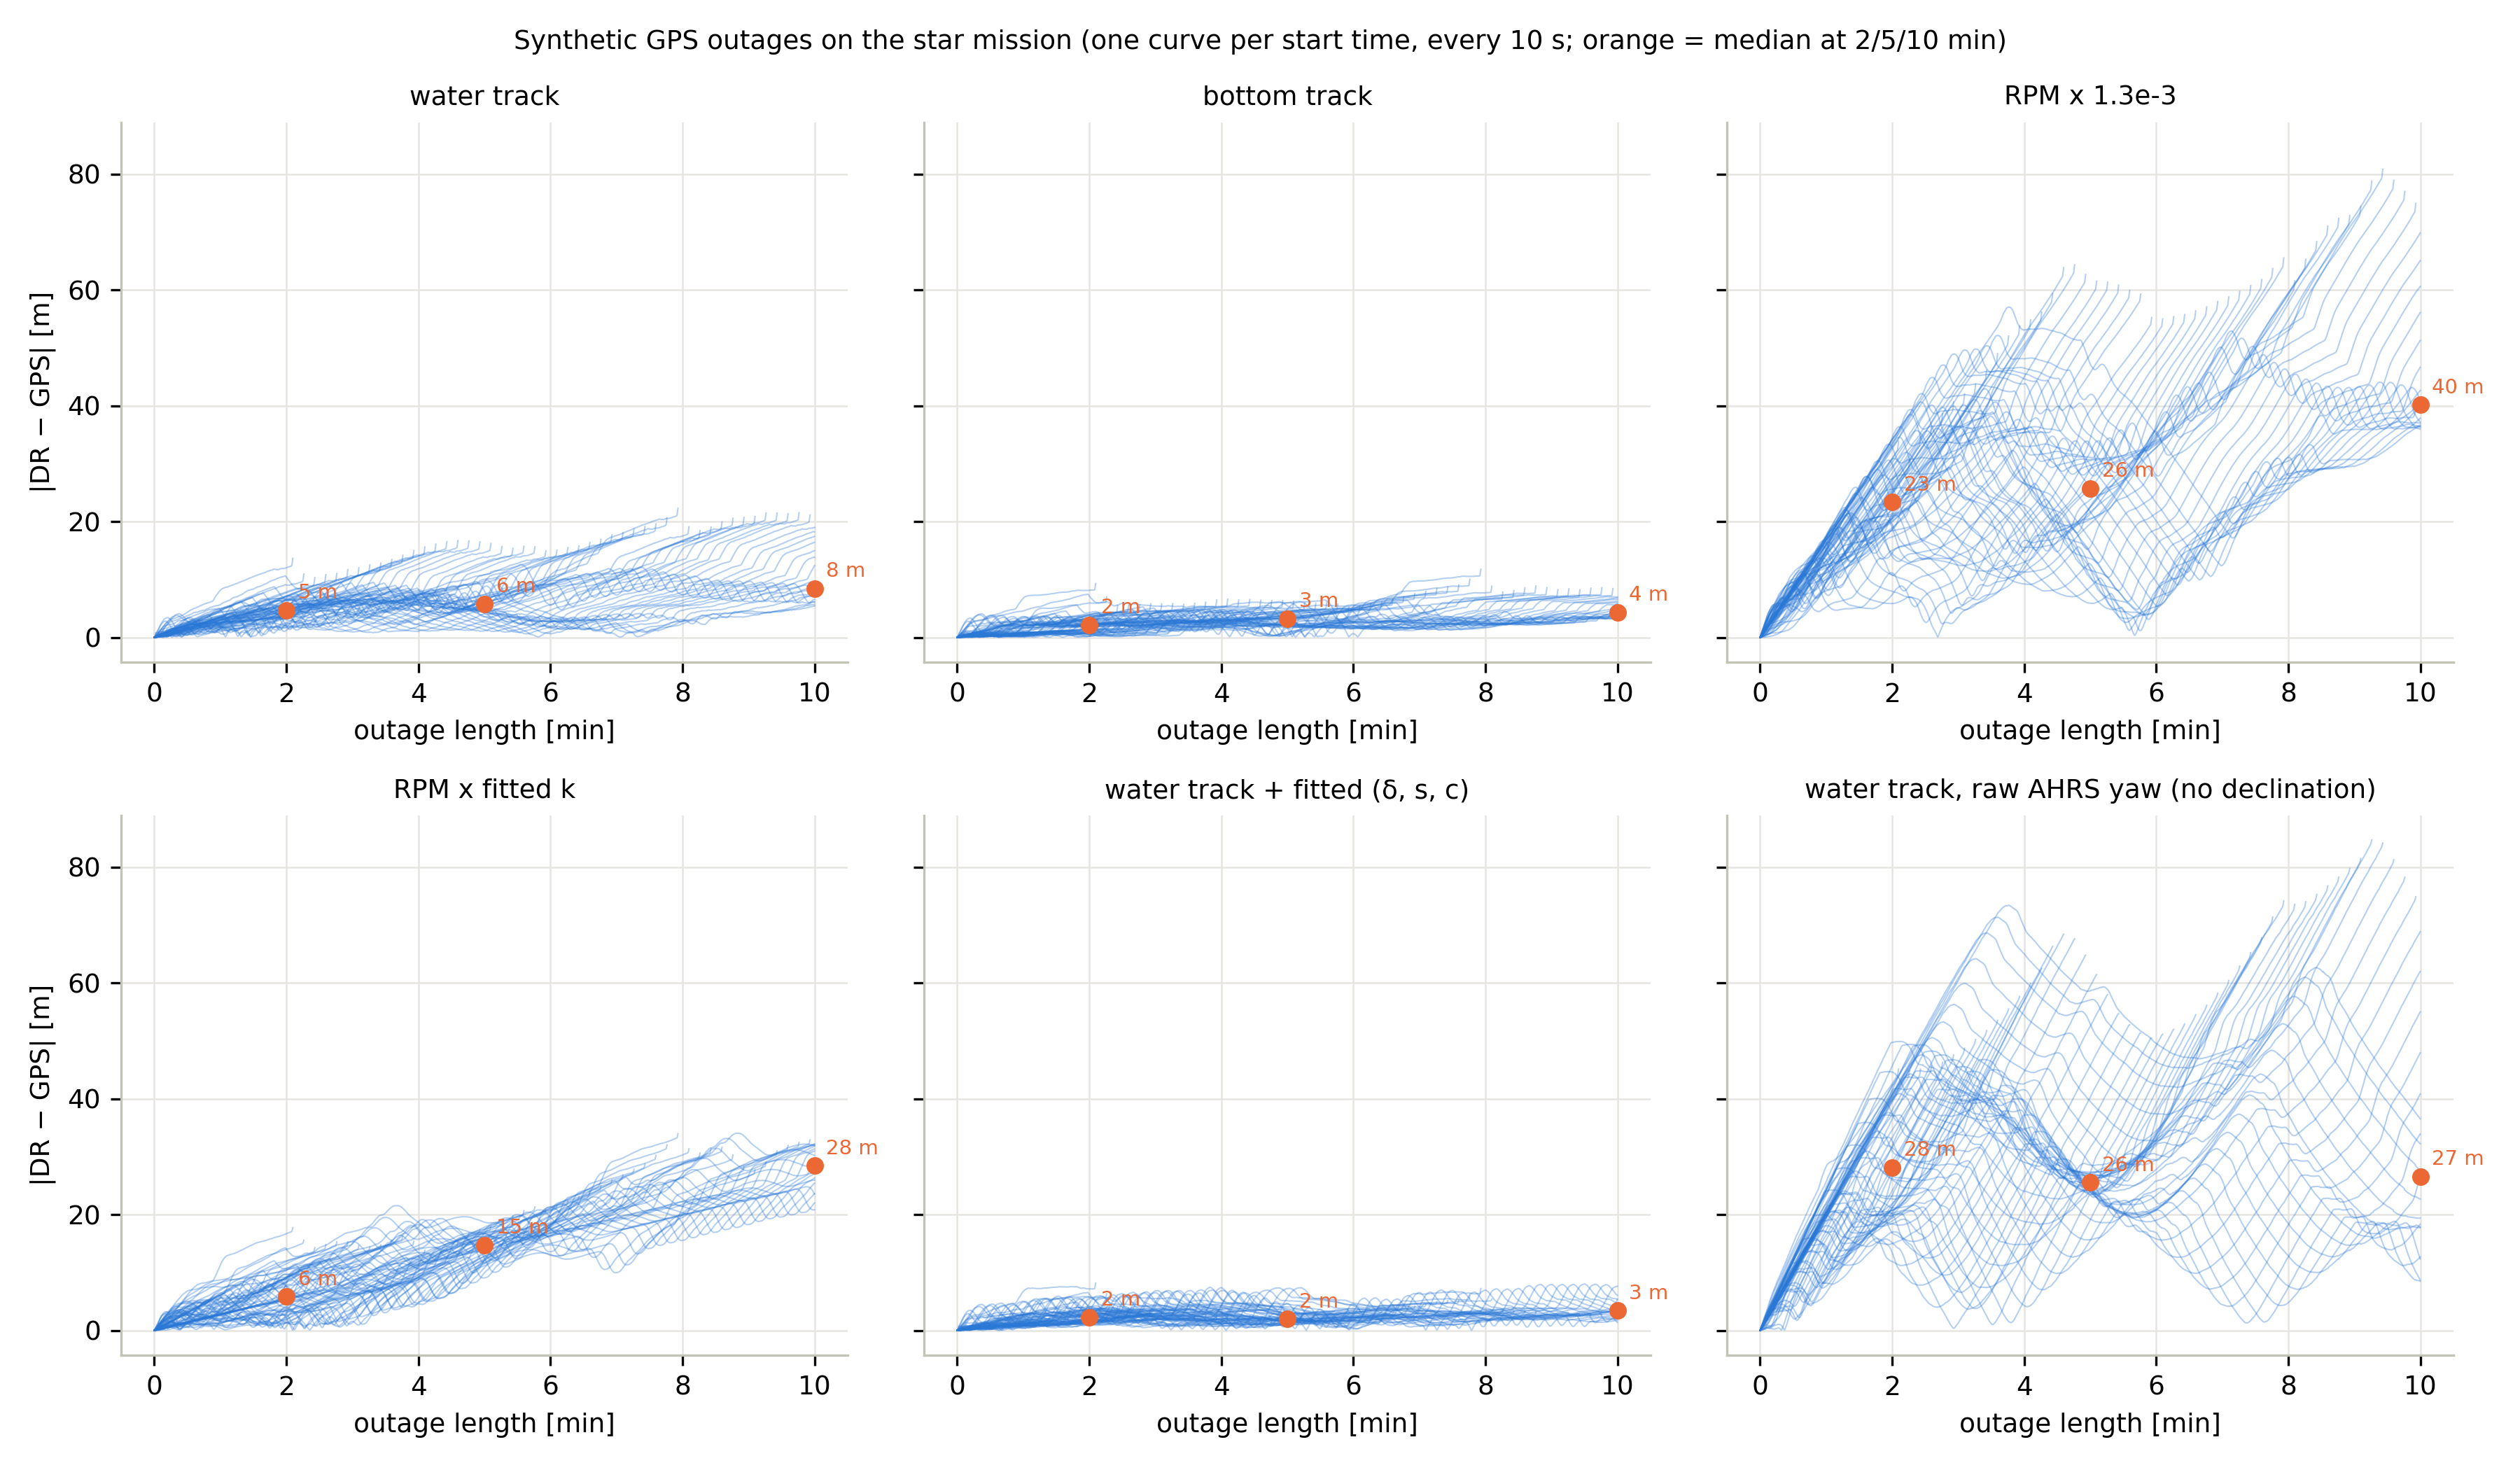
\includegraphics[width=0.62\textwidth]{star_outage_drift}
\caption{Drift of dead reckoning restarted every \SI{10}{\second} on the star, one curve per start time, for six speed and heading sources. Orange dots are the medians at \SIlist{2;5;10}{\minute}.}
\label{fig:drift}
\end{figure*}

\subsection{Calibration on simulations}

On \num{1000} held-out simulations with 500 posterior draws each, the rank histograms (Fig.~\ref{fig:sbc}) are close to uniform. The largest deviation of the rank ECDF from uniform is between 0.024 and 0.037 for the five parameters, below the 95\,\% critical value of 0.043 for \num{1000} draws, and the central 50\,\% and 90\,\% intervals contain the truth in 50--52\,\% and 92--94\,\% of cases. The mean 90\,\% width is \SI{14.5}{\degree} for $\delta$ against \SI{27}{\degree} for the prior, 0.123 against 0.27 for $s$, \SI{0.23}{\meter\per\second} against 0.72 for each current component, and 0.21 against 1.53 decades for $\sigma_v$. Heading bias is the least constrained, because it is unobservable without GPS: for the dive windows its posterior is \SI{27.9}{\degree} wide, the width of the prior. The first noise model gave the same picture (coverage 91--94\,\%; ECDF deviations 0.023--0.049). Calibration on the simulator therefore says nothing about the gap between the simulator and the vehicle, which the next subsections test.

\begin{figure*}[t]
\centering
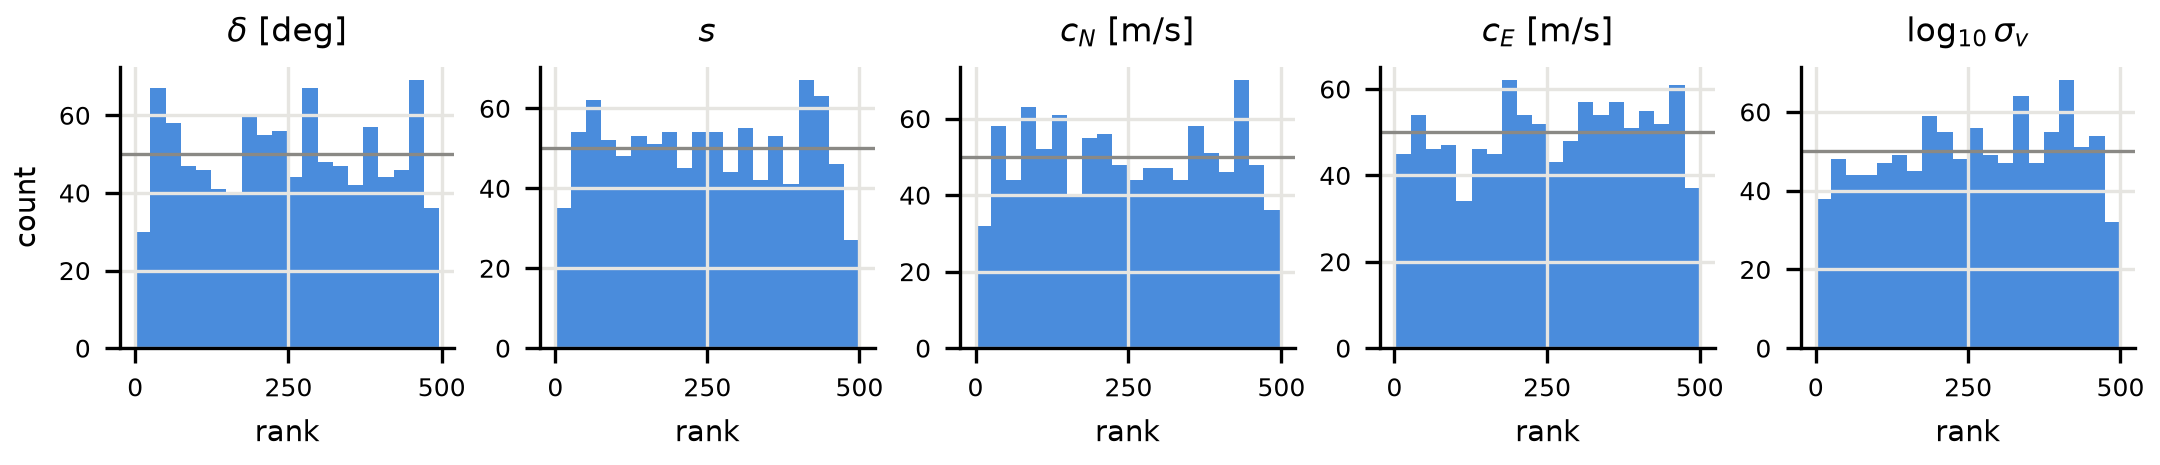
\includegraphics[width=0.72\textwidth]{sbc_ranks}
\caption{Simulation-based calibration of the amortized posterior: rank of the true parameter among 500 posterior draws for \num{1000} held-out simulations (20 bins; grey line: uniform expectation).}
\label{fig:sbc}
\end{figure*}

\subsection{Real star windows: the first noise model and its replacement}
\label{sec:v1v2}

Table~\ref{tab:v1v2} compares the posterior on the 23 real star windows with the all-leg reference of Table~\ref{tab:fits} for both noise models. With the first, the posterior was narrow and displaced: $\delta = \SI{-1.04}{\degree}$ (90\,\% interval $-1.62$ to $-0.46$) against $+0.09^{\circ} \pm 0.16^{\circ}$, and the intervals contained the reference in only 22, 70, 57 and 61\,\% of windows for $\delta$, $s$, $c_N$ and $c_E$. The cause is in the noise model. On the real star the DVL bottom and water track agree to \SI{0.03}{\meter\per\second} per axis, while GPS and DVL velocity disagree by \SI{0.15}{\meter\per\second}; at the settings of the first model the simulated GPS--DVL disagreement was \SIrange{0.06}{0.10}{\meter\per\second}, and the real DVL noise lay below the lower bound of the prior of $\sigma_v$. The network could plausibly represent a GPS--DVL discrepancy of that size only as a bias or a current. Making the two noise levels broad nuisances (Section~III) reduced the displacement of $\delta$ to $\SI{-0.55}{\degree}$ (interval $-1.51$ to $+0.42$) and raised the containment to 52, 65, 78 and 52\,\%. The intervals are still narrower than the errors: the median $|z|$ of the posterior mean against the reference is 1.6, 0.9, 0.8 and 1.5, where a calibrated Gaussian gives 0.67.

\begin{table}[t]
\caption{Posterior on the 23 real star windows against the all-leg reference: median over windows of the posterior mean and of the 90\,\% interval, and the number of windows whose 90\,\% interval contains the reference. v1: first noise model; v2: broad noise nuisances.}
\label{tab:v1v2}
\centering
\scriptsize
\setlength{\tabcolsep}{1.6pt}
\begin{tabular}{@{}lrcrcr@{}}
\toprule
 & Ref. & v1 mean [90\,\%] & in & v2 mean [90\,\%] & in \\
\midrule
$\delta$ [$^\circ$] & $+0.09$ & $-1.04$ [$-1.62,-0.46$] & 5 & $-0.55$ [$-1.51,+0.42$] & 12 \\
$s$ & 0.965 & 0.975 [0.956, 0.994] & 16 & 0.972 [0.952, 0.991] & 15 \\
$c_N$ [m/s] & $+0.003$ & $+0.011$ [$-0.004,+0.032$] & 12 & $-0.004$ [$-0.026,+0.012$] & 18 \\
$c_E$ [m/s] & $-0.019$ & $-0.034$ [$-0.053,-0.010$] & 14 & $-0.031$ [$-0.059,-0.010$] & 12 \\
\bottomrule
\end{tabular}
\end{table}

Part of the remaining discrepancy lies in the reference, not in the posterior. Bottom track and GPS velocity are both over-ground, so the angle that turns the heading-rotated bottom-track vector onto the GPS vector is the heading bias of a window, whatever the current or the scale. Computed for each of the 23 windows it varies between $-2.6^{\circ}$ and $+3.4^{\circ}$ (standard deviation $1.25^{\circ}$) with the heading of the window (Fig.~\ref{fig:hbias}), as a magnetic compass deviation does. The posterior mean of $\delta$ follows it with a correlation of 0.93 and an rms difference of $0.58^{\circ}$, which is about the noise of the window-level estimate itself (about $0.5^{\circ}$), and the window-level value lies inside the 90\,\% interval in 21 of 23 windows (91\,\%). The single constant of the all-leg fit averages this variation out. This check was added after the under-coverage had been seen and uses the same data, so it explains, and does not prove, that the under-coverage in $\delta$ is mostly a reference problem; no window-level reference exists for $s$ and $\vect{c}$, for which the containment of 65 and 52--78\,\% stands unexplained.

\begin{figure}[t]
\centering
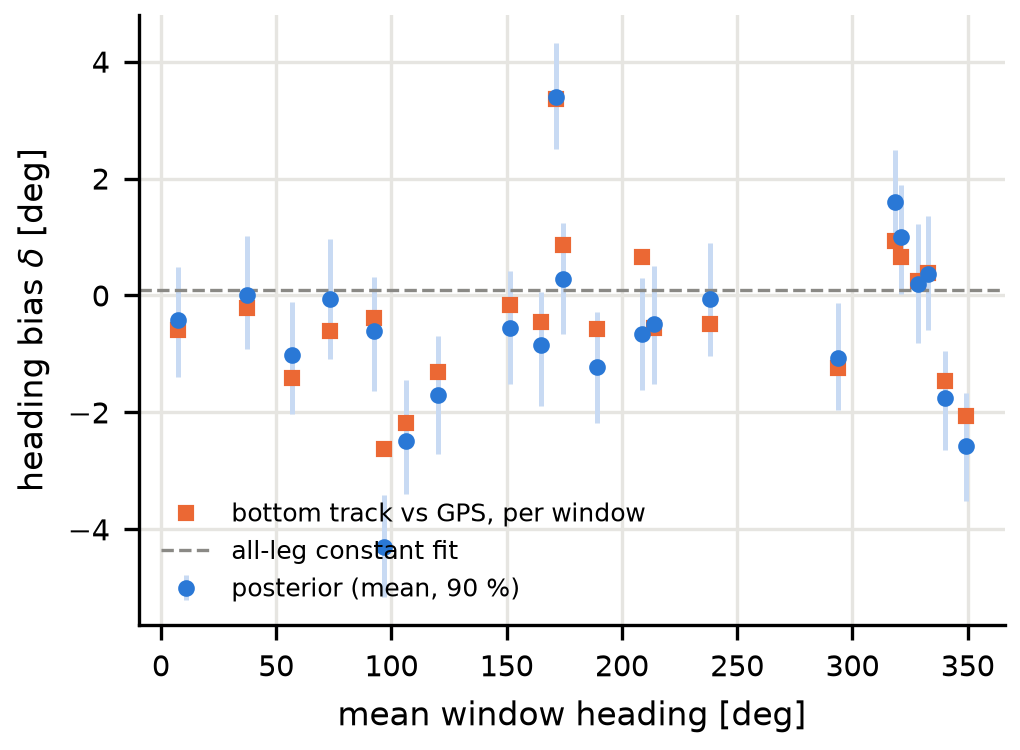
\includegraphics[width=0.88\columnwidth]{heading_bias_check}
\caption{Heading bias per star window: posterior (mean and 90\,\% interval) and the independent estimate from bottom track versus GPS, against the mean heading of the window. The dashed line is the constant all-leg fit.}
\label{fig:hbias}
\end{figure}

Identifiability behaves as the model predicts. In the one window whose heading varies by less than \SI{20}{\degree}, the 90\,\% widths of the current magnitude and of the scale are 0.19 and \SI{0.22}{\meter\per\second} and 0.22, against 0.064 and 0.069 for the 22 windows containing a turn, while the width of $\delta$ is unchanged (\SI{1.95}{\degree} against \SI{1.91}{\degree}). The heading bias stays observable on a straight leg because bottom track and GPS are both over-ground velocities; the current and the scale are confounded along the track. One window is an anecdote. The posterior-predicted drift of the nominal water-track dead reckoning over the window has a median of \SI{4.6}{\meter} against \SI{4.8}{\meter} observed, the observed drift lies inside the 90\,\% predictive interval in 65\,\% of windows, and the correlation across windows is 0.44.

\subsection{Propagation through the sidescan dive}

The onboard estimate at the moment of the first GPS fix accepted after the \SI{34}{\minute} dive was \SI{19.9}{\meter} from that fix (\SI{16.3}{\meter} north, \SI{11.4}{\meter} east; the fix itself had a horizontal accuracy estimate of \SI{10}{\meter}), i.e. \SI{0.73}{\percent} of the \SI{2.73}{\kilo\meter} path. An independent dead reckoning from the last accepted fix before the dive, using the filter's heading and the DVL water track, closes \SI{23.3}{\meter} off; with bottom track \SI{41.5}{\meter}. The two endpoint fixes carry \SI{13}{\meter} and \SI{10}{\meter} accuracy estimates, so, taking the accuracy estimates as one standard deviation, the closure of the water-track dead reckoning is $23 \pm 16$\,m, and the three numbers are consistent with each other. The filter's own reported position standard deviation at the end of the dive was \SI{1.0}{\meter}, an order of magnitude below the observed error, which illustrates why a filter covariance is not an error budget.

Which parameters may be carried from the star to the dive? The heading bias and the speed scale are properties of the vehicle and its sensors; the current is a property of the site and the day, and the sidescan survey was flown about \SI{50}{\kilo\meter} from the star, a day later. Two propagations are therefore compared (Table~\ref{tab:prop}). In variant A all three parameters are drawn from the star posteriors, which is the naive use. In variant B the heading bias comes from the star, where it is observable, and the scale and the current come from the posteriors of the dive's own windows, in which bottom track is present and GPS is absent, applied window by window; the windows are either drawn independently (a lower bound on the spread) or at the same posterior quantile in every window (an upper bound).

\begin{table}[t]
\caption{Predicted error of the nominal water-track dead reckoning at resurfacing of the sidescan dive (\SI{34.2}{\minute}), median and 90\,\% interval, and the percentile of the observed closure of \SI{23.3}{\meter} in the predicted distribution.}
\label{tab:prop}
\centering
\footnotesize
\begin{tabular}{@{}lccc@{}}
\toprule
Variant & median [m] & 90\,\% [m] & obs.\ percentile \\
\midrule
A: all from the star & 94 & 18--333 & 7\,\% \\
B: $(s,\vect{c})$ from dive, indep. & 56 & 49--64 & 0\,\% \\
B: same, correlated & 83 & 53--176 & 0\,\% \\
\bottomrule
\end{tabular}
\end{table}

\begin{figure*}[t]
\centering
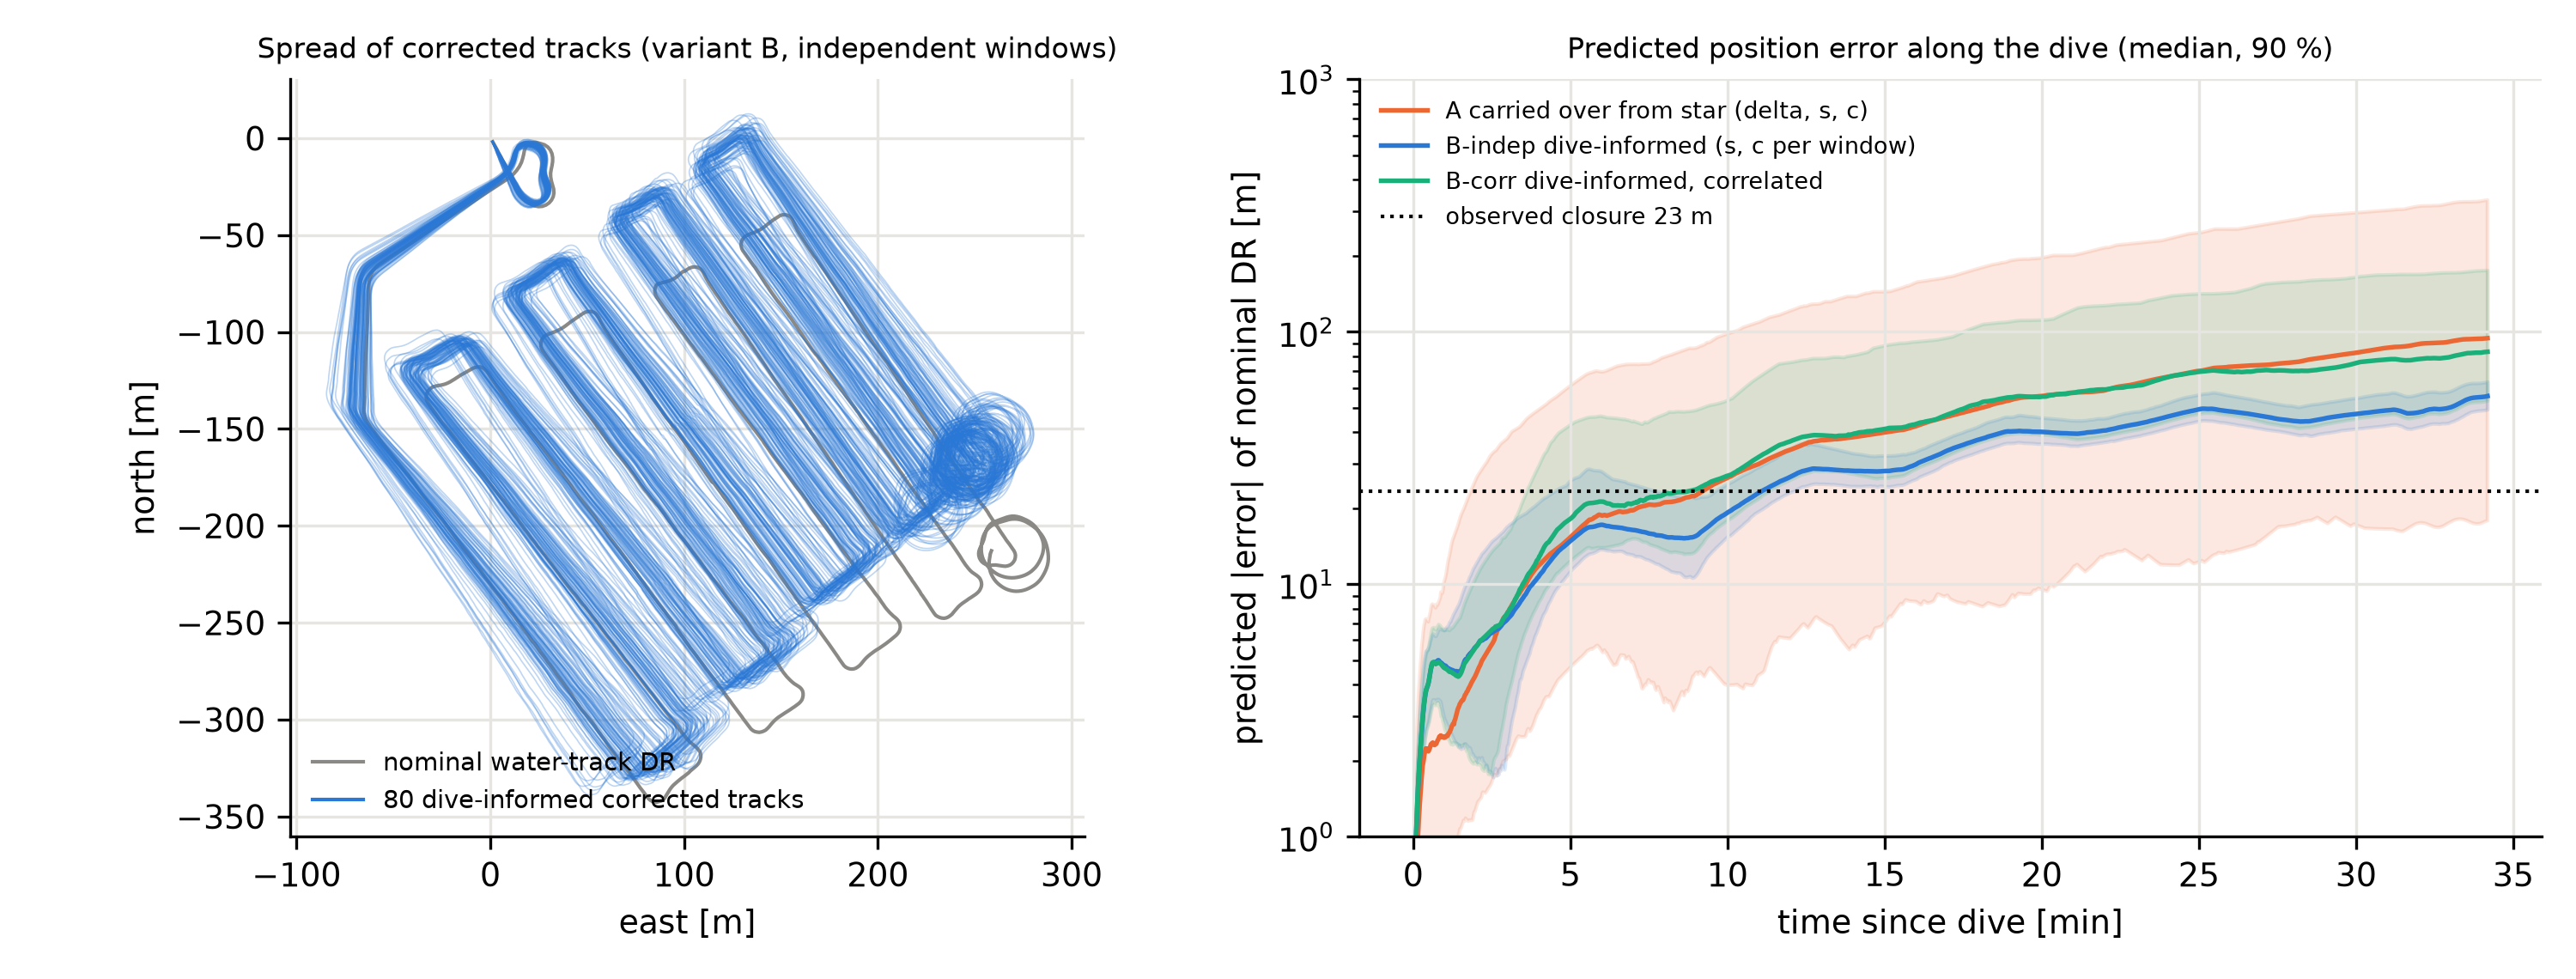
\includegraphics[width=0.72\textwidth]{sidescan_envelope}
\caption{Sidescan dive of 8 September 2026. Left: nominal water-track dead reckoning (grey) and 80 corrected tracks drawn from the dive-informed posterior (variant B, independent windows). Right: predicted error of the nominal dead reckoning along the dive for the three variants (median and 90\,\% envelope); the dotted line is the observed closure of \SI{23}{\meter}.}
\label{fig:envelope}
\end{figure*}

Variant A predicts \SI{94}{\meter} (90\,\%: 18--333), which contains the observed closure at its 7th percentile; most of it is the star's current of \SI{0.03}{\meter\per\second}, which accumulates to \SI{64}{\meter} over \SI{34}{\minute}, and it is right for the wrong reason. Variant B gives \SI{56}{\meter} (49--64) with independent windows and \SI{83}{\meter} (53--176) with correlated windows; the observed \SI{23}{\meter} lies below both intervals. The dive-window posteriors have a median current of $(+0.020, -0.008)$\,\si{\meter\per\second} and a median scale of 0.974, and a current of \SI{0.02}{\meter\per\second} alone accumulates \SI{43}{\meter} in \SI{34}{\minute}. The observed closure is $23 \pm 16$\,m, so the prediction overshoots by about two endpoint standard deviations. With one dive it cannot be decided whether the posterior is overconfident about the current by \SIrange{0.01}{0.02}{\meter\per\second}, or whether the net current was smaller than the window-wise values because a tidal current reversed within \SI{34}{\minute}, which a piecewise-constant model would still represent as a sequence of non-zero windows. The envelope of Fig.~\ref{fig:envelope} is therefore not validated by this dive, and the posterior is not shown to be calibrated over long submerged intervals.

\subsection{A second vehicle and the misspecification test}

Thor differs from Marie in every respect that matters: no bottom lock, a water track that the DVL itself flagged invalid, an older DUNE version and a propeller-driven filter. Its six surface windows lie on nearly parallel headings, and the posterior of $\delta$ from them is correspondingly wide, $\SI{-5.1}{\degree}$ (90\,\%: $-15.1$ to $+4.9$) against a least-squares value of $\SI{-3.9}{\degree}$ from the same runs, and contains the reference in 4 of 6 windows; the posterior of the scale contains the reference (0.984) in all six. The least-squares fit itself confounds $\delta$ and the current on such headings. Its two dives closed \SI{224}{\meter} and \SI{298}{\meter} off in water-track dead reckoning (the onboard, propeller-based filter was \SI{292}{\meter} and \SI{341}{\meter} off, and its own log claimed \SI{0.6}{\meter} and \SI{0.5}{\meter} because that diagnostic is evaluated after the correction).

\begin{table}[t]
\caption{Thor's dives: predicted error of the nominal water-track dead reckoning at resurfacing (median and 90\,\% interval, in metres) with $\delta$ from Thor's surface windows and $(s,\vect{c})$ from the dive's own windows (79 windows in total), and the observed closure of the same dead reckoning with its percentile in the predicted distribution.}
\label{tab:thor}
\centering
\footnotesize
\setlength{\tabcolsep}{3pt}
\begin{tabular}{@{}lcccc@{}}
\toprule
Dive & Obs. & Indep. windows & Correl. windows & Percentile \\
\midrule
1 (\SI{19.0}{\minute}) & 224 & 185 (35--440) & 260 (67--681) & 63 / 40\,\% \\
2 (\SI{24.7}{\minute}) & 298 & 236 (70--604) & 397 (92--758) & 60 / 32\,\% \\
\bottomrule
\end{tabular}
\end{table}

Propagating the posteriors through the two dives (Table~\ref{tab:thor}) gives predicted errors of \SI{185}{\meter} and \SI{236}{\meter} with independent windows and \SI{260}{\meter} and \SI{397}{\meter} with correlated windows, and the observed closures lie inside every 90\,\% interval, at the 32nd to 63rd percentile. Where the data do not constrain the heading bias, the posterior says so and the predicted error range contains the truth. The test is lenient, because the intervals span more than an order of magnitude (\SIrange{35}{758}{\meter}); it shows that the posterior is not confidently wrong here, not that it predicts Thor's error well.

\begin{table}[t]
\caption{Mahalanobis test in summary space: threshold \num{61.6} (99th percentile of held-out simulations; their median 31.1). Windows flagged out of the total, with the first noise model in brackets.}
\label{tab:detect}
\centering
\footnotesize
\begin{tabular}{@{}lccc@{}}
\toprule
Window set & $n$ & median $d^2$ & flagged \\
\midrule
Marie star & 23 & 25.2 & 0 (0) \\
Marie star, raw magnetic heading & 23 & 34.3 & 0 (0) \\
Marie sidescan dive & 64 & 31.5 & 0 (0) \\
Thor surface & 6 & 45.7 & 1 (2) \\
Thor dives & 79 & 28.8 & 0 (2) \\
\bottomrule
\end{tabular}
\end{table}

The Mahalanobis test (Table~\ref{tab:detect}) does not separate Thor from Marie: one of six Thor surface windows and none of 79 Thor dive windows exceed the threshold, and the median distance of the star windows is below that of the simulations. The reason is that, with wide priors on $\delta$, $s$ and $\vect{c}$ and with GPS and bottom track randomly absent, the simulator covers all these windows; Thor's dive windows look like simulated windows without GPS and bottom track, with parameters inside the prior. For the same reason the raw-heading windows are not flagged: they are not outside the training distribution, they are inside it with a large $\delta$, and the posterior says so, with $\delta = +12.09^{\circ}$ (90\,\%: $+11.01$ to $+13.04$) against the $12.72^{\circ}$ that the onboard filter adds ($12.81^{\circ}$ from the fit of Table~\ref{tab:fits}; 14 of 23 windows contain the latter). The over-narrow posterior of the first noise model was not flagged either (0 of 23 windows). A distance in a 32-dimensional summary space is therefore not a sufficient safeguard here; the checks that found the problems were comparisons with independent references and predicted-versus-observed closures.



%% ===========================================================================
\section{Discussion}

\paragraph{What the results support} The amortized posterior is calibrated on the simulator, identifies the heading bias of a two-minute surface window well enough to follow a compass deviation that varies by several degrees with heading, recovers the \SI{12.7}{\degree} heading offset when it is left in the raw heading, and widens where the data are uninformative, as the wide posterior on Thor's parallel-heading windows and the predicted errors of Table~\ref{tab:thor} show. A pipeline using the raw heading would learn a bias of \SI{12.7}{\degree}, or call it a current.

\paragraph{What they do not support} On real windows the intervals are narrower than the errors against the constant references (52--78\,\% containment against a nominal 90\,\%), and the first noise model shows how strongly the posterior depends on nuisance settings that calibration on simulations cannot test. The propagated envelope over-predicts the sidescan closure by about two endpoint standard deviations, from a single dive. The misspecification test in summary space flagged neither the second vehicle nor the failure of the first noise model. The posterior should therefore be treated as a calibration aid for surface windows, not as a predictor of underwater error.

\paragraph{Vehicle-level and site-level parameters} The heading bias and the speed scale are properties of the vehicle and its sensors and may be carried from a calibration to a survey; the current belongs to the site and the day and must not be. The carried-over variant of Table~\ref{tab:prop} looks better than the dive-informed variants only because its interval (\SIrange{18}{333}{\meter}) is wide.

\paragraph{A constant heading bias is too simple} The per-window bias of Fig.~\ref{fig:hbias} has the shape of a magnetic deviation curve. The natural extension is to replace $\delta$ by a low-order harmonic function of the heading, which the star, with its six headings, can constrain and the sidescan lawnmower, with two, cannot separate from a constant; the posterior width on the sidescan windows would then reflect that. Whether it reduces the sidescan overshoot is untested.

\paragraph{Limits} The current during the star was indistinguishable from zero at the \SI{0.02}{\meter\per\second} level, so the posterior over $\vect{c}$ is validated only as consistent with zero. There is one sidescan dive, closed against a \SI{10}{\meter} fix; further dives from the same day and the surface log that followed would turn this comparison into a validation set. No ultra-short-baseline fix reached any vehicle, so all position truth is standalone GPS. Neighbouring windows overlap by \SI{75}{\percent}, so the coverage figures from 23 windows are uncertain by several windows, and the window-level heading reference was computed after the results were seen.

\paragraph{Relation to conventional calibration} The least-squares fits of Table~\ref{tab:fits} are the classical method \cite{kinsey2007alignment} and remain the reference. The amortized posterior adds an uncertainty from a short window without a dedicated manoeuvre and a per-window heading bias; it does not yet add a safeguard against a wrong noise model, for which the comparison with independent references was indispensable.

%% ===========================================================================
\section{Conclusion}
%% ===========================================================================

A summary network and a normalizing flow trained on a kinematic simulator return calibrated posteriors over heading bias, speed scale, current and velocity noise on simulated windows (90\,\% intervals contain the truth in 92--94\,\% of cases) and follow the per-window heading bias of a real surface star pattern (correlation 0.93 with an independent estimate, 21 of 23 windows inside the 90\,\% interval), revealing a heading-dependent compass bias of $-2.6^{\circ}$ to $+3.4^{\circ}$ that a constant-bias calibration averages out. Against constant references the real-window intervals are too narrow, and a first noise model was overconfident until GPS and bottom-track noise were made broad nuisances. Carried through a \SI{34}{\minute} sidescan dive the posterior predicts \SIrange{56}{83}{\meter} of error at resurfacing where $23 \pm 16$\,m was observed, so it is not yet a validated predictor of underwater error; for a second vehicle without bottom lock, whose dives closed \SI{224}{\meter} and \SI{298}{\meter} off, its wide predicted intervals contain both closures. A Mahalanobis test in summary space flagged neither that vehicle nor the first noise model's failure. The next steps are a heading-dependent bias model, more dives from the same vehicle to turn the dive comparison into a validation set, and a misspecification test that acts on the posterior and on predicted closures, not on the summary distance alone.

\section*{Acknowledgment}
Field data were collected during the AT-334/834 course of the University Centre in Svalbard with NTNU AUR-Lab vehicles and the UNIS boats \emph{Hanna Resvoll}, \emph{Silas} and \emph{Kolga}. \todo{add funding and group members if required.}

\bibliographystyle{IEEEtran}
\bibliography{refs}

\end{document}
